\documentclass[11pt]{article}
%prepared in AMSLaTeX, under LaTeX2e
\addtolength{\oddsidemargin}{-.75in} 
\addtolength{\evensidemargin}{-.75in}
\addtolength{\topmargin}{-.6in}
\addtolength{\textwidth}{1.4in}
\addtolength{\textheight}{1.3in}

\renewcommand{\baselinestretch}{1.06}

\usepackage{fancyvrb,xspace}
\usepackage{palatino,amsmath,amssymb,amsthm}
\usepackage[final]{graphicx}
\usepackage[pdftex, colorlinks=true, plainpages=false, linkcolor=blue, citecolor=red, urlcolor=blue]{hyperref}

% macros
\newcommand{\RR}{\mathbb{R}}
\newcommand{\grad}{\nabla}
\newcommand{\lam}{\lambda}
\newcommand{\ds}{\displaystyle}
\newcommand{\Matlab}{\textsc{Matlab}\xspace}


\title{POPDIP: a POsitive-variables \\ Primal-Dual Interior Point optimization method}
\author{Ed Bueler}
\date{\today}

\begin{document}
\maketitle

\begin{abstract}
The algorithm here is an example of the Newton-type primal-dual interior point algorithms in \cite[Algorithm 16.1, section 16.7]{GrivaNashSofer2009} and \cite{YamashitaYabe1996}.  It minimizes a smooth nonlinear function subject to the constraints that all the variables are nonnegative, plus linear equality constraints:
\begin{equation}
\begin{matrix}
\text{minimize} \qquad   & f(x) \\
\text{subject to} \qquad & A x = b \\
                         & x \ge 0
\end{matrix} \label{eq:problem}
\end{equation}

This is a specialized algorithm for nonnegativity constraints $x\ge 0$, and it is not suitable for general inequality constraints of the form ``$g_i(x)\ge 0$.''  Nor is it suitable for general equality constraints ``$g_i(x)=0$.''  However, it can be used as an interior-point method for linear programming in the case where $f(x)=c^\top x$, though it has no special performance improvements for that case.

These short notes are \emph{not} research.  I simply implement a special case of a well-known algorithm.  Furthermore ``POPDIP'' is a name I made up; it is not in common use.  However, I am interested in this class of methods because local quadratic convergence, seen in unconstrained Newton algorithms, can be proven.  This property is much harder to achieve for constrained problems.
\end{abstract}

\thispagestyle{empty}

\bigskip
\subsection*{Introduction}

First consider a nonlinear optimization problem with only nonnegativity (informally: positivity) constraints on the variables:
\begin{equation}
\begin{matrix}
\text{minimize} \qquad & f(x) \\
\text{subject to} \qquad & x \ge 0
\end{matrix} \label{eq:posproblem}
\end{equation}
As usual, ``$x\ge 0$'' in \eqref{eq:posproblem} means that each entry of $x\in\RR^n$ is nonnegative.  The feasible set for \eqref{eq:posproblem} is the convex and closed set $S = \{x\in \RR^n\,:\,x\ge 0\}$, with interior $S^\circ = \{x\in \RR^n\,:\,x > 0\}$, and $f:S \to \RR$ is a continuous and smooth function.

The next section will address the general problem \eqref{eq:problem} including linear equality constraints.

One can derive an interior point method by considering a logarithmic barrier function \cite[section 16.2]{GrivaNashSofer2009}.  Let $\mu>0$ be a (temporarily) fixed constant.  If $x\in S^\circ$ then the following function is well-defined:
\begin{equation}
\beta_\mu(x) = f(x) - \mu \sum_{i=1}^n \ln x_i \label{eq:posbarrierfunction}
\end{equation}
Let $\{e_1,\dots,e_n\}$ be the standard basis of $\RR^n$.  The first-order necessary condition for the \emph{unconstrained} problem of minimizing $\beta_\mu$, namely $\grad \beta_\mu(x)=0$ for $x \in S^\circ$, is
\begin{equation}
\grad f(x) - \mu \sum_{i=1}^n \frac{1}{x_i} e_i = 0 \label{eq:posfirstorderbarrier}
\end{equation}

Conditions \eqref{eq:posfirstorderbarrier} can be reformulated by defining additional variables
    $$\lambda_i = \frac{\mu}{x_i}$$
so that $\lambda\in\RR^n$.  Note that $\lambda>0$ if and only if $x>0$ because $\lambda_i x_i = \mu > 0$.  Then \eqref{eq:posfirstorderbarrier}, plus feasibility for $x$, is equivalent to the following nonlinear system of equations and inequalities:
\begin{align}
\grad f(x) - \lambda &= 0 \label{eq:posfirstordersystem} \\
\lambda_i x_i &= \mu, \qquad i=1,\dots,n \notag \\
x &\ge 0 \notag \\
\lambda &\ge 0 \notag
\end{align}
The feasible set for $x$ and for $\lambda$ is the same, namely $S \subset \RR^n$.   (By contrast, for a general primal-dual interior point method, specifically Algorithm 16.1 in \cite[section 16.7]{GrivaNashSofer2009}, the feasible set for the primal variables $x$ is different from that of the dual variables $\lambda$.)  Because of the second condition in \eqref{eq:posfirstordersystem}, both $x$ and $\lambda$ are strictly positive and thus in the interior $S^\circ$.

The first condition in \eqref{eq:posfirstordersystem} can be rewritten using a Lagrangian function for \eqref{eq:posproblem}:
\begin{equation}
\mathcal{L}(x,\lambda) = f(x) - \sum_{i=1}^n \lambda_i x_i.  \label{eq:poslagrangian}
\end{equation}
Now \eqref{eq:posfirstordersystem} states that $\grad_x \mathcal{L}(x,\lambda)=0$.  In fact, the KKT conditions \cite[sections 14.4, 14.5]{GrivaNashSofer2009} of \eqref{eq:posproblem} are nearly the same as \eqref{eq:posfirstordersystem} but with the second equation replaced by complementarity,
\begin{align}
\grad f(x) - \lambda &= 0 \label{eq:poskkt} \\
\lambda_i x_i &= 0, \qquad i=1,\dots,n \notag \\
x &\ge 0 \notag \\
\lambda &\ge 0 \notag
\end{align}

Thus the barrier method which generated system \eqref{eq:posfirstordersystem} modifies KKT conditions \eqref{eq:poskkt} by changing complementary slackness condition into a nonzero connection between the primal and dual variables, in which their product is set to a positive constant.  System \eqref{eq:posfirstordersystem} describes a solution which is interior to the feasible set, and thus is different from the solution to \eqref{eq:poskkt}.

The first condition in \eqref{eq:poskkt} allows $\lambda$ to be eliminated if desired: $\lambda = \grad f(x)$.  Writing the KKT conditions without these dual variables gives a \emph{nonlinear complementarity problem} (NCP) \cite{FacchineiPang2007},
\begin{equation}
x \ge 0, \qquad \grad f(x) \ge 0, \qquad x_i (\grad f(x))_i = 0.  \label{eq:posncp}
\end{equation}
Thus we may regard POPDIP as solving the $\mu$-modified NCP
\begin{equation}
x \ge 0, \qquad \grad f(x) \ge 0, \qquad x_i (\grad f(x))_i = \mu. \label{eq:mumodifiedncp}
\end{equation}
However, the method achieves quadratic convergence substantially because it updates primal and dual variables separately.  Stating the algorithm or the original KKT conditions as an NCP, thereby suppressing the dual variables, is not beneficial.  Note that such NCP formulations also appear in problems which are not optimizations, rather variational inequalities, including in a glaciological case upon which I am focussed \cite{Bueler2016}.


\subsection*{General problem}

Suppose from now on that $f:\RR^n \to \RR$ is twice continuously-differentiable.  Let $A\in\RR^{m\times n}$, $m\le n$, be a full rank matrix, and suppose $b\in\RR^m$.  The POPDIP algorithm solves general problems of form \eqref{eq:problem} in the abstract, restated here:
\begin{equation}
\begin{matrix}
\text{minimize} \qquad   & f(x) \\
\text{subject to} \qquad & A x = b \\
                         & x \ge 0
\end{matrix} \tag{1}
\end{equation}

Observe that the constraints are in standard form for linear programming (LP) problems \cite[chapter 4]{GrivaNashSofer2009}.  If $f(x)=c^\top x$ for some fixed $c\in\RR^n$ then \eqref{eq:problem} is an LP problem in standard form, and then POPDIP becomes an LP interior point method, though one with no special adaptations to that case; compare e.g.~\cite{ZhangTapiaDennis1992}.

The (primal) feasible set is
\begin{equation}
S = \{Ax=b \text{ and } x\ge 0\} \subset \RR^n.  \label{eq:primalfeasible}
\end{equation}
The iterates $x_k$ from our algorithm will be in the interior,\footnote{In general, $S^o$ is not the topological interior of $S \subset \RR^n$, which is empty when equality constraints apply ($m>0$).} defined to be
\begin{equation}
S^o = \{Ax=b \text{ and } x > 0\} \subset \RR^n.  \label{eq:primalinterior}
\end{equation}
We will assume that $S^o$ is nonempty and that a feasible iterate in $S^o$ can be found.  (In fact the user will \emph{not} need to provide an initial iterate which is feasible with respect to ``$Ax=b$'', but they will need to provide a strictly-positive initial iterate.)

Consider the following Lagrangian for \eqref{eq:problem}:
\begin{equation}
\mathcal{L}(x,\tau,\lambda) = f(x) - \tau^\top (Ax - b) - \lambda^\top x, \label{eq:lagrangian}
\end{equation}
for multipliers $\tau\in\RR^m$ and $\lambda\in \RR^n$.  Function \eqref{eq:lagrangian} reduces to \eqref{eq:poslagrangian} if there are $m=0$ linear equality constraints (so $\tau$ is absent).  The first-order necessary conditions, the KKT conditions, for \eqref{eq:problem} are given by $\grad_x\mathcal{L}=0$ and $\grad_\tau\mathcal{L}=0$, plus complementarity for the primal variables $x$ and dual variables $\lambda$:
\begin{align}
\grad f(x) - A^\top \tau - \lambda &= 0 \label{eq:kkt} \\
-A x + b &= 0 \notag \\
\lambda_i x_i &=0, \qquad i=1,\dots,n \notag \\
x &\ge 0 \notag \\
\lambda &\ge 0 \notag
\end{align}
Conditions \eqref{eq:kkt} reduce to system \eqref{eq:poskkt} given in the Introduction when there are $m=0$ linear equality constraints.


\subsection*{Algorithm design}

The POPDIP algorithm solves \eqref{eq:problem} by applying a Newton method to a $\mu$-modified form of KKT conditions \eqref{eq:kkt}.  The modification replaces complementarity $\lambda_i x_i = 0$ by the conditions
\begin{equation}
\lambda_i x_i = \mu_k, \qquad i=1,\dots,n \notag \\
\end{equation}
for a (scalar) barrier sequence $\{\mu_k>0\}$ which will to zero.  Thus POPDIP computes primal and dual iterates in the interior: $x,\lambda \in S^o$.  However, if the method converges as $\mu_k \to 0$ then the limiting values of $x$ and $\lambda$ solve the KKT conditions \eqref{eq:kkt}.  Though the algorithm is terminated after a finite number of steps, in examples the KKT system is solved to high accuracy.

Each step of the algorithm is a Newton step for the modified equalities from \eqref{eq:kkt}, namely
\begin{align}
\grad f(x) - A^\top \tau - \lambda &= 0 \label{eq:equalities} \\
-A x + b &= 0 \notag \\
\lambda_i x_i &= \mu_k, \qquad i=1,\dots,n \notag
\end{align}
Because of its third equation, \eqref{eq:equalities} is always a nonlinear system.  However, if $f$ is quadratic or linear then \emph{only} the third equation, the modified complementarity condition, is nonlinear.

Intuitively, an interior-point iteration for \eqref{eq:equalities} sees ``changing equations'' with iteration $k$.  As we update the $\mu_k$ value, each new iterate is attempting to solve new equations.  Thus, though the iterates of POPDIP should converge to the solution of KKT problem \eqref{eq:kkt}, they will not converge to a solution of \eqref{eq:equalities} for any particular $\mu_k>0$.

The Newton step computes a search direction in the $x,\tau,\lambda$ variables using the linearization of equations \eqref{eq:equalities}.  The actual POPDIP step is subject to positivity constraints on $x$ and $\lambda$, via a ratio test \cite[section 3.1]{GrivaNashSofer2009}, uses generally different step sizes for the three parts $x,\tau,\lambda$.

To describe the Newton step in detail, let $x=x_k+\Delta x$, $\tau=\tau_k+\Delta\tau$ and $\lambda=\lambda_k+\Delta\lambda$.  The unknowns form a candidate search direction $p=(\Delta x,\Delta\tau,\Delta\lambda)$ which is modified later.  Substituting into \eqref{eq:equalities} and expanding to first order gives
\begin{align}
\grad f(x_k) + \grad^2 f(x_k) \Delta x - A^\top \tau_k - A^\top \Delta \tau - \lambda_k - \Delta \lambda &= 0 \label{eq:prenewtonstep} \\
-A x_k - A \Delta x + b &= 0 \notag \\
(\lambda_k)_i (x_k)_i + (x_k)_i (\Delta\lambda)_i + (\lambda_k)_i (\Delta x)_i &= \mu_k, \qquad i=1,\dots,n \notag
\end{align}
Rearranging this as a vectorized and matrix-block system gives
\begin{equation}
\begin{bmatrix}
\grad^2 f(x_k) & -A^\top & -I \\
-A             & 0       & 0  \\
\Lambda_k      & 0       & X_k
\end{bmatrix}
\begin{bmatrix}
\Delta x \\
\Delta \tau \\
\Delta \lambda
\end{bmatrix}
=
\begin{bmatrix}
-\grad f(x_k) + A^\top \tau_k + \lambda_k \\
A x_k - b \\
\mu_k e - \Lambda_k x_k
\end{bmatrix}. \label{eq:newtonstep}
\end{equation}
Here $I$ is the $n\times n$ identity matrix, $e=(1,1,\dots,1)^\top \in \RR^n$, and we have defined $n\times n$ diagonal matrices from the primal/dual vectors $x,\lambda\in\RR^n$:
    $$X = \begin{bmatrix} x_1 & & \\ & \ddots & \\ & & x_n \end{bmatrix}, \qquad \Lambda = \begin{bmatrix} \lambda_1 & & \\ & \ddots & \\ & & \lambda_n \end{bmatrix}.$$
Note that $\Lambda x = X \lambda$ in this notation.\footnote{The product $\Lambda x = X\lambda$ is simply \, \texttt{x.*lambda}\, in \Matlab.}

Linear system \eqref{eq:newtonstep} can also be written as
\begin{equation}
M p = - r \label{eq:overallnewtonstep}
\end{equation}
where $M$ is the $(2n+m) \times (2n+m)$ square, sparse \emph{system matrix} on the left side of \eqref{eq:newtonstep} and $r=r_k(x_k,\tau_k,\lambda_k) \in \RR^{2n+m}$ is the residual of system \eqref{eq:equalities} for the current iterate, using the \emph{residual function}
\begin{equation}
r_k(x,\tau,\lambda) = \begin{bmatrix}
\grad f(x) - A^\top \tau - \lambda \\
- A x + b \\
\Lambda x - \mu_k e
\end{bmatrix}. \label{eq:residualnewtonstep}
\end{equation}

We will solve system \eqref{eq:newtonstep}, equivalently \eqref{eq:overallnewtonstep}, using direct linear algebra, via Matlab's default ``$\backslash$'' linear solver.  Because this direct solver is quite accurate, the residual norm $\|b-A x_k\|$, part of the right-hand side of \eqref{eq:newtonstep}, will be very small.  In this sense, system \eqref{eq:newtonstep} imposes the classical null-space requirement on the search direction for linear equality constraints \cite[chapter 3]{GrivaNashSofer2009}:
\begin{equation}
A \Delta x = 0.  \label{eq:dxnull}
\end{equation}
On the other hand, use of a direct solver means the implementation is not scalable to large problem sizes.  A scalable implementation would not assemble the full matrix $M$ in \eqref{eq:overallnewtonstep}, and it might use an iterative solver, along the way exploiting the sparse block structure of $M$ including the symmetry of its upper-left $2\times 2$ block.  Preconditioners \cite{Bueler2021} for the $\grad^2 f(x_k)$ block and the equality-constraint Schur complement \cite[chapters 14]{Bueler2021} should be considered.

Given a solution $(\Delta x,\Delta\tau,\Delta\lambda)$ of \eqref{eq:newtonstep}, the update formulas are
\begin{align}
x_{k+1} &= x_k + \alpha_x \Delta x \label{eq:updates} \\
\tau_{k+1} &= \tau_k + \alpha_\tau \Delta \tau \notag \\
\lambda_{k+1} &= \lambda_k + \alpha_\lambda \Delta \lambda \notag
\end{align}
Separate step sizes $\alpha_x,\alpha_\tau,\alpha_\lambda$ are used for the three vector variables $x,\tau,\lambda$, though this is not the only choice \cite{YamashitaYabe1996}.  Because the constraint equations are linear, the full Newton step $\alpha_\tau=1$ is always used for the $\tau$ multipliers.

The quadratic convergence of a general primal-dual interior point method is proven in subsection 16.7.2 of \cite{GrivaNashSofer2009}.  That method replaces general inequality constraints $g_i(x)\ge 0$ by $g_i(x) - s_i =0$, with slack variables $s_i\ge 0$.  However, in our case this replacement says $x_i-s_i=0$ and $s_i\ge 0$, clearly unneeded as it simply renames existing primal variables $x$.

Also, the back-tracking globalization of the inequality constraints described in Algorithm 16.1 of \cite{GrivaNashSofer2009}, choosing $\alpha_x$ from $\{1,1/2,1/4,\dots\}$ so that $g_i(x_k + \alpha_x \Delta x) > 0$ for all $i$, is not needed to maintain feasibility of our primal variables because of the linearity of all of the constraint functions in \eqref{eq:problem}.  That is, for constraints $Ax=b$ and $x\ge 0$ a ratio test for $\Delta x$ will guarantee primal feasibility, as also holds in the simplex method \cite[chapter 5]{GrivaNashSofer2009}.

On the other hand, just like in Algorithm 16.1 in \cite{GrivaNashSofer2009}, our optimization algorithm shortens the step in the Newton search direction \emph{only} because of the inequality constraints, and not for the ``usual'' (unconstrained) line search reasons, for instance to generate sufficient decrease by an Armijo or Wolfe rule \cite[section 11.5]{GrivaNashSofer2009}.  In this sense our method is most suitable for quadratic functions $f(x)$, and it may need additional refinements for more general, especially non-convex, objective functions.  It should be used with caution if the Hessian $\grad^2 f(x)$ varies significantly during the iteration.

POPDIP determines step sizes $\alpha_x,\alpha_\lambda$ for the inequality-constrained primal and dual variables via a condition of (strict) positivity for $x_{k+1}$ and $\lambda_{k+1}$.  Suppose $0<\kappa<1$.  For the primal variables, assuming $x_k\in S^o$ so that $x_k>0$, we require that for all $i$ such that $(\Delta x)_i < 0$,
\begin{equation}
(x_k)_i + \alpha_x (\Delta x)_i \ge (1-\kappa) (x_k)_i \qquad \iff \qquad \alpha_x \le - \kappa \frac{(x_k)_i}{(\Delta x)_i}. \label{eq:preratio}
\end{equation}
(If $(\Delta x)_i \ge 0$ then $(x_k)_i + \alpha_x (\Delta x)_i \ge (1-\kappa) (x_k)_i$ automatically.)  Rule \eqref{eq:preratio} is applied with $\kappa \approx 1$, so that the inequality constaints are nearly activated, and also with a preference for the Newton step $\alpha_x=1$.  A similar ratio test applies to the dual variables and determines $\alpha_\lambda$.  In summary:
\begin{align}
\alpha_x &= \min_{1\le i\le n} \left\{1, \,-\kappa \frac{(x_k)_i}{(\Delta x)_i} \,:\, (\Delta x)_i < 0\right\}, \label{eq:ratiotests} \\
\alpha_\tau &= 1, \notag \\
\alpha_\lambda &= \min_{1\le i\le n} \left\{1, \,-\kappa \frac{(\lambda_k)_i}{(\Delta \lambda)_i} \,:\, (\Delta \lambda)_i < 0\right\}. \notag
\end{align}
(Compare subsection 16.7.2 in \cite{GrivaNashSofer2009}.)

The optimality test in POPDIP requires that a certain merit function associated to system \eqref{eq:equalities} be smaller than a given tolerance, either in an absolute sense or relative to the initial value of the merit function.  We use a merit function which is a norm of the residual \eqref{eq:residualnewtonstep}:
\begin{equation}
    \nu(x,\tau,\lambda) = \max\{\|\grad f(x)-A^\top \tau - \lambda\|_2,\|b-Ax\|_2,\|\Lambda x\|_2\}.  \label{eq:meritfunction}
\end{equation}
This function is fundamentally the same as in section 16.7 of \cite{GrivaNashSofer2009}, but adapted to our problem.  (Recall that we expect $\|b-Ax_k\|=0$ to good accuracy after the initial step.)  Note that in the limit $\mu_k\to 0$ we have $\nu(x_*,\tau_*,\lambda_*) = 0$ for the exact solution of \eqref{eq:equalities}.  On the other hand, for some $\mu_k > 0$ the exact solution of \eqref{eq:equalities} would give a value $\nu(x_*,\tau_*,\lambda_*)=\sqrt{n}\, \mu_k>0$.

Subsection 16.7.2 of \cite{GrivaNashSofer2009} describes how Algorithm 16.1 should be modified so that, by Theorem 16.17, the algorithm will exhibit the local quadratic convergence.  The Theorem requires a specific scheme for $\mu_k$, and a specific choice for $\kappa$ in ratio tests \eqref{eq:ratiotests}.  In our case these are the equations
\begin{align}
\mu_k &= \min\{\theta \nu(x_k,\tau_k,\lambda_k),\nu(x_k,\tau_k,\lambda_k)^2\}, \label{eq:muupdate} \\
\kappa &= \max\{\bar\kappa,1-\nu(x_k,\tau_k,\lambda_k)\}, \label{eq:kappaformula}
\end{align}
for parameters $0<\theta<1$ and $0<\bar\kappa<1$.  We choose the default values of the parameters as $\theta=0.1$ and $\bar\kappa=0.9$, based on the minimal hints in Example 16.16 in \cite{GrivaNashSofer2009}.

The method by which the initial dual variables are determined (below) is a somewhat ad hoc construction for which I have no reference, but compare \cite{Gertzetal2004}.


\subsection*{Pseudocode}

We now present a pseudocode for POPDIP.  The defaults for parameters are $\text{\texttt{rtol}}=10^{-4}$, $\text{\texttt{atol}}=10^{-50}$, $\text{\texttt{maxiters}}=200$, $\theta=0.1$, and $\bar\kappa=0.9$.

\bigskip
\noindent \textsc{Algorithm POPDIP.}
\begin{quote}
\begin{itemize}
\item[\emph{inputs}]  smooth function $f:\RR^n\to\RR$; user code returns $f(x)$, $\grad f(x)$, and $\grad^2 f(x)$
\item[]  full (row) rank matrix $A$ of size $m\times n$ with $0\le m\le n$
\item[]  vector $b\in\RR^m$
\item[]  primal initial values (vector) $x_0\in\RR^n$ such that $x_0 > 0$
\item[\emph{parameters}]  $\text{\texttt{rtol}}>0$
\item[]  $\text{\texttt{atol}}>0$
\item[]  $\text{\texttt{maxiters}}>0$
\item[]  $0<\theta<1$
\item[]  $0<\bar\kappa<1$
\item[\emph{output}]  an estimate $(x_k,\tau_k,\lambda_k)$ of the solution to \eqref{eq:problem} and \eqref{eq:kkt}
\item  determine initial dual variables:
    \renewcommand{\labelenumi}{(\roman{enumi})}
    \begin{enumerate}
    \item $\tau_0 = 0$
    \item $g_0 = \grad f(x_0)$
    \item if $g_0 \le 0$ then $\mu_0=1$; otherwise $\mu_0$ is average of those products $(x_0)_i (g_0)i$ where $(g_0)_i > 0$
    \item $(\lambda_0)_i = \mu_0 / (x_0)_i$ for $i=1,\dots,n$
    \end{enumerate}
\item  for $k=0,1,2,\dots,\text{\texttt{maxiters}}-1$
    \renewcommand{\labelenumi}{(\roman{enumi})}
    \begin{enumerate}
    \item evaluate gradient $g_k = \grad f(x_k)$
    \item evaluate merit function of \eqref{eq:kkt}:
    $$\nu_k = \max\{\|g_k-A^\top \tau_k - \lambda_k\|_2,\|b-Ax_k\|_2,\|\Lambda_k x_k\|_2\}$$
    \item optimality test: if $\nu_k<\text{\texttt{atol}}$ or $\nu_k<(\text{\texttt{rtol}})\, \nu_0$ then stop
    \item evaluate barrier parameter: $\mu_k = \min\{\theta \nu_k,\nu_k^2\}$
    \item compute Newton step by solving linear system \eqref{eq:newtonstep} for $(\Delta x,\Delta \tau,\Delta \lambda)$:
    $$\begin{bmatrix}
\grad^2 f(x_k) & -A^\top & -I \\
-A             & 0       & 0  \\
\Lambda_k      & 0       & X_k
\end{bmatrix}
\begin{bmatrix}
\Delta x \\
\Delta \tau \\
\Delta \lambda
\end{bmatrix}
=
\begin{bmatrix}
-g_k + A^\top \tau_k + \lambda_k \\
A x_k - b \\
\mu_k e - \Lambda_k x_k
\end{bmatrix}$$
    \item evaluate ratio test parameter: $\kappa = \max\{\bar\kappa,1-\nu_k\}$
    \item apply ratio tests for step sizes, to keep $x_{k+1},\lambda_{k+1}$ positive:
\begin{align*}
\alpha_x &= \min_{1\le i\le n} \left\{1, \,-\kappa \frac{(x_k)_i}{(\Delta x)_i} \,:\, (\Delta x)_i < 0\right\} \\
\alpha_\tau &= 1 \\
\alpha_\lambda &= \min_{1\le i\le n} \left\{1, \,-\kappa \frac{(\lambda_k)_i}{(\Delta \lambda)_i} \,:\, (\Delta \lambda)_i < 0\right\}
\end{align*}
    \item update to the next iterate:
\begin{align*}
x_{k+1} &= x_k + \alpha_x \Delta x \\
\tau_{k+1} &= x_k + \alpha_\tau \Delta x \\
\lambda_{k+1} &= \lambda_k + \alpha_\lambda \Delta \lambda
\end{align*}
    \end{enumerate}
\end{itemize}
\end{quote}


\subsection*{\Matlab implementation}

The POPDIP algorithm is implemented by a \Matlab code \href{https://github.com/bueler/popdip/blob/main/matlab/popdip.m}{\texttt{popdip.m}}.  If one wants to accept the default parameter values then the signature is

\medskip
\centerline{\texttt{function [x,tau,lam] = popdip(x0,f,A,b)}}

\medskip
\noindent where \texttt{x} $\in\RR^n$, \texttt{tau} $\in\RR^m$, \texttt{lam} $\in\RR^n$ are approximations of the solution to \eqref{eq:kkt}.  The user-provided function \texttt{f} has signature

\medskip
\centerline{\texttt{function [fx,dfx,Hfx] = f(x)}}

\medskip
\noindent where \texttt{fx} $\in\RR$ is the objective value, \texttt{dfx} $\in\RR^n$ is the gradient, and \texttt{Hfx} $\in\RR^{n\times n}$ is the Hessian.

For more control the POPDIP parameters can be set to non-default value as follows:

\medskip
\centerline{\texttt{popdip(x0,f,A,b,rtol,atol,maxiters,theta,kappabar)}}

\medskip
\noindent The parameters have the default values listed in the last section.

Additional diagnostic outputs can be requested by using more output arguments:

\medskip
\centerline{\texttt{[x,tau,lam,iteratelist,nuklist,muklist] = popdip(\dots)}}

\medskip
\noindent If \texttt{iteratelist} is not requested then none of \texttt{iteratelist,nuklist,muklist} are saved.

Download the \href{https://github.com/bueler/popdip/blob/main/matlab/popdip.m}{\texttt{popdip.m}} code, this documentation, and the example codes demonstrated in the next section, from the Github repository:
\begin{center}
    \href{https://github.com/bueler/popdip}{\texttt{github.com/bueler/popdip}}
\end{center}


\subsection*{Examples}

\subsubsection*{Example 1.}

We first try a small 2D test problem in \href{https://github.com/bueler/popdip/blob/main/matlab/small.m}{\texttt{small.m}}, which is a positivity-constrained quadratic minimization:
\begin{equation}
\begin{matrix}
\text{minimize} \qquad & f(x) = \frac{1}{2} (x_1-1)^2 + \frac{1}{2} (x_2+1)^2 \\
\text{subject to} \qquad & x \ge 0
\end{matrix} \label{eq:smallproblem}
\end{equation}
The unconstrained minimum is the infeasible point $\hat x =(1,-1)^\top$.  A sketch shows that the exact solution of the constrained problem is $x_*=(1,0)^\top$.

Running with the given initial iterate $x_0=(2,2)^\top$ and \texttt{rtol} $=10^{-14}$, and otherwise using the default parameters in POPDIP, gives strongly superlinear, and possibly quadratic, convergence:
\begin{Verbatim}[fontsize=\footnotesize]
>> small
        x_1                  x_2                  nu_k                 mu_k
  0:    2.000000000000000    2.000000000000000    5.656854249492381
  1:    1.641421356237309    0.641421356237310    1.488944443027284    0.565685424949238
  2:    1.245446520462486    0.245446520462486    0.432311672017441    0.148894444302728
  3:    1.069404818969903    0.069404818969903    0.104965543876699    0.043231167201744
  4:    1.013447008853577    0.013447008853577    0.019272663285475    0.010496554387670
  5:    1.000537794151783    0.000537794151783    0.000760964805668    0.000371435550115
  6:    1.000000867357066    0.000000867357066    0.000001226629190    0.000000579067435
  7:    1.000000000002257    0.000000000002257    0.000000000003192    0.000000000001505
  8:    1.000000000000000    0.000000000000000    0.000000000000000    0.000000000000000
\end{Verbatim}
Both the merit function values $\nu_k$ and the barrier parameters $\mu_k$ go rapidly to zero.  The iterates $x_k$ are graphed in the following figure.

\bigskip
\begin{center}
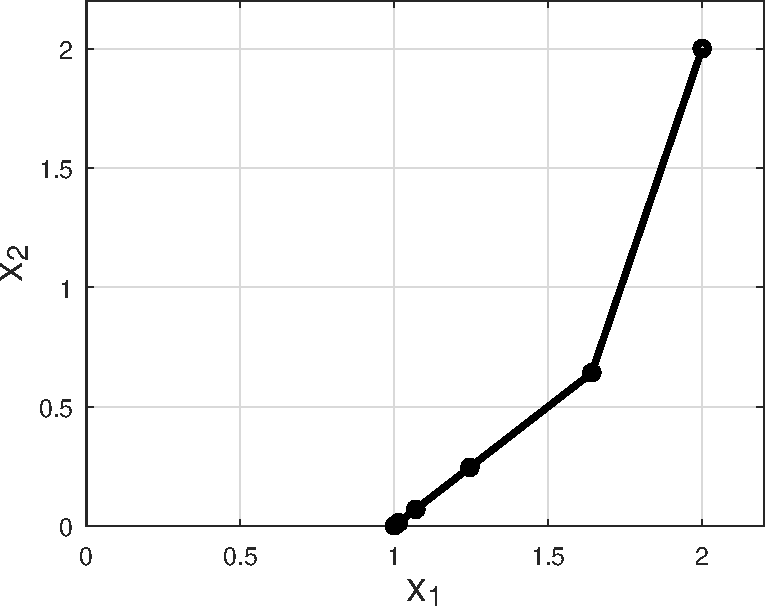
\includegraphics[width=0.5\textwidth]{figs/small.pdf}
\end{center}


\subsubsection*{Example 2.}

The next problem is an $n=5$ linear programming (LP) problem, in standard form, with $m=3$ linear equality constraints:
\begin{equation}
\begin{matrix}
\text{minimize} \qquad & f(x) = c^\top x \\
\text{subject to} \qquad & A x = b \\
 & x \ge 0
\end{matrix} \label{eq:linearproblem}
\end{equation}
where $\ds c = \begin{bmatrix} -1 & -2 & 0 & 0 & 0 \end{bmatrix}^\top$, $\ds A = \begin{bmatrix} -2 & 1 & 1 & 0 & 0 \\ -1 & 2 & 0 & 1 & 0 \\ 1 & 0 & 0 & 0 & 1 \end{bmatrix}$, and $\ds b = \begin{bmatrix} 2 & 7 & 3 \end{bmatrix}^\top$.  The same problem is solved by the simplex method in \cite[section 5.2]{GrivaNashSofer2009}, where the solution is found on the third iteration starting from the basic feasible solution $x=0$.  The standard-form problem arises from the LP problem
\begin{equation}
\begin{matrix}
\text{minimize} \qquad & z = -x_1 - 2x_2 \\
\text{subject to} \qquad & -2x_1 + x_2 \le 2 \\
 & -x_1 + 2x_2 \le 7 \\
 & x_1 \le 3 \\
 & x_1, x_2 \ge 0
\end{matrix} \label{eq:twodlp}
\end{equation}
which can be easily sketched.

The standard-form LP problem is defined in a short driver program \href{https://github.com/bueler/popdip/blob/main/matlab/linear.m}{\texttt{linear.m}}.  It runs POPDIP with initial iterate $x_0=(1,1,1,1,1)^\top$ and \texttt{rtol} $=10^{-14}$, otherwise using the default parameters.  The result is strongly superlinear convergence similar to Example 1:
\begin{Verbatim}[fontsize=\footnotesize]
>> linear
        x_1                  x_2                  nu_k                 mu_k
  0:    1.000000000000000    1.000000000000000    5.477225575051662
  1:    1.749124060578910    3.650175187884218    2.662463982283214    0.547722557505166
  2:    2.771966360502739    4.813544496010846    0.673064121890067    0.266246398228321
  3:    2.977196636050274    4.937189711618397    0.151356274478520    0.067306412189007
  4:    2.993139910878286    4.988863175677374    0.033061726195566    0.015135627447852
  5:    2.999412769621014    4.999167116475287    0.002445966295331    0.001093077739031
  6:    2.999996717485349    4.999995406776724    0.000013394027090    0.000005982751118
  7:    2.999999999901378    4.999999999862158    0.000000000401658    0.000000000179400
  8:    3.000000000000000    5.000000000000000    0.000000000000000    0.000000000000000
\end{Verbatim}

The 2D iterates $x_k$ are graphed below.  This looks like the ideal performance of an interior-point method on an LP problem.  Compare figure 5.1, chapter 10, and section 10.6 in \cite{GrivaNashSofer2009}.

\bigskip
\begin{center}
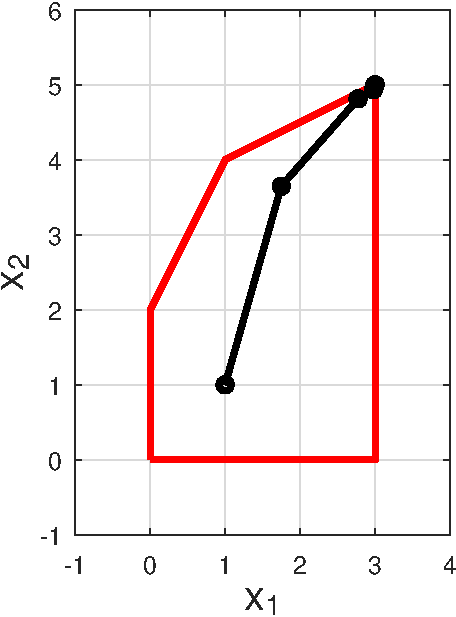
\includegraphics[width=0.35\textwidth]{figs/linear.pdf}
\end{center}

It is worth considering the Newton step \eqref{eq:newtonstep} in this LP case.  Because the objective function $f(x) = c^\top x$ is linear, the gradient is constant and the Hessian is zero:
\begin{equation}
\begin{bmatrix}
0         & -A^\top & -I \\
-A        & 0       & 0  \\
\Lambda_k & 0       & X_k
\end{bmatrix}
\begin{bmatrix}
\Delta x \\
\Delta \tau \\
\Delta \lambda
\end{bmatrix}
=
\begin{bmatrix}
-c + A^\top \tau_k + \lambda_k \\
A x_k - b \\
\mu_k e - \Lambda_k x_k
\end{bmatrix}. \label{eq:lpnewtonstep}
\end{equation}

Perhaps surprisingly, given that a positive-definite leading block has disappeared, compared to the quadratic minimization case, the square system matrix $M$ on the left of \eqref{eq:lpnewtonstep} is invertible when $\mu_k>0$.  (See the proof in the Appendix which uses the facts that $A$ has full row rank and $\mu_k\ne 0$.)  Thus it is okay that in Example 2 the \href{https://github.com/bueler/popdip/blob/main/matlab/linear.m}{\texttt{linear.m}} code supplies a zero Hessian.

When one measures the conditioning of $M$ in practice, it actually holds steady as $\mu_k\to 0$.  This is something I do not see how to prove.


\subsubsection*{Example 3.}

FIXME obstacle problem in 1D: \href{https://github.com/bueler/popdip/blob/main/matlab/obstacle.m}{\texttt{obstacle.m}}

\begin{equation}
    f[u] = \int_0^1 \frac{1}{2} |u'(x)|^2 - q(x) u(x)\,dx \label{obstaclefunctional}
\end{equation}

$\Delta x = 1 / (n+1)$
\begin{equation}
    f(u) = \Delta x \sum_{i=0}^n \left(\frac{1}{2} \left(\frac{u_{i+1}-u_i}{\Delta x}\right)^2 - q(x_{i+1/2}) \frac{u_i + u_{i+1}}{2}\right) \label{obstacleobjective}
\end{equation}
where $u_0=0$ and $u_{n+1}=0$ when they appear

gradient components for $i=1,\dots,n$
\begin{equation}
\grad f(u)_i = \frac{1}{\Delta x} \left\{\begin{matrix}
2 u_1 - u_2 & (i=1) \\
-u_{i-1} + 2 u_i - u_{i+1} & (1<i<n) \\
-u_{n-1} + 2 u_n & (i=n) \\
\end{matrix} \right\} - \frac{\Delta x}{2} (q(x_{i-1/2}) + q(x_{i+1/2}))
\end{equation}

Hessian matrix
\begin{equation}
\grad^2 f(u) = \frac{1}{\Delta x} \begin{bmatrix}
2  & -1 &    &    \\
-1 &  2 & -1 &    \\
   &    & \ddots &\\
   &    & -1 &  2
\end{bmatrix}
\end{equation}

\subsection*{Possible improvements}

FIXME

We may consider possible improvements of our algorithm.  First, in Algorithm 16.1 the computation of the Newton search direction is followed by separate line searches in $x$ and in $\lambda$.  These line searches only maintain nonnegativity and they do not seek sufficient decrease of $f(x)$; they only use ratio tests.  Secondly, equation \eqref{eq:newtonstep} can be symmetrized by multiplying the second half of the equations by $-\Lambda^{-1}$:
\begin{equation}
\begin{bmatrix}
\grad^2 f(x) & - I \\
-I & - \Lambda^{-1} X
\end{bmatrix}
\begin{bmatrix}
\Delta x \\
\Delta \lambda
\end{bmatrix}
=
\begin{bmatrix}
-\grad f(x) + \lambda \\
x - \mu_k \Lambda^{-1} e
\end{bmatrix}
 \label{eq:symmnewtonstep}
\end{equation}

FIXME further simplify into system of $n$ equations for $\lambda$ only

These facts suggests two possible changes:
\begin{enumerate}
\item Back-tracking line search is appropriate as a globalization even for unconstrained optimization.  Thus there must be cases where it is appropriate for problem \eqref{eq:problem} as well.  Once the ratio tests are applied, further back-tracking could be used based on sufficient decrease.  Compare the modified back-tracking line searches in \cite{BensonMunson2006}.
\item One can replace linear system \eqref{eq:newtonstep} with symmetrized system \eqref{eq:symmnewtonstep}.
\end{enumerate}
Determining if these are actual improvements would require testing which we have not done.


%\subsection*{Application to example problem (\texttt{glacier}).}
%FIXME a primal-dual interior point method for a glacier problem appears in \cite{Calvoetal2003}

\medskip

\bibliography{doc}
\bibliographystyle{siam}

\appendix
\subsection*{Appendix: Invertibility of the system matrix in LP cases.}

The square system matrix $M$ on the left of \eqref{eq:lpnewtonstep} is invertible.

\begin{proof}  If $\mu_k>0$ then $x_k,\lambda_k$ are strictly positive so the diagonal matrices $\Lambda_k,X_k$ are (trivially) invertible.  If $Mp=0$ for $p=(\Delta x,\Delta \tau,\Delta \lambda)$ then, by the first equation in \eqref{eq:lpnewtonstep}, $\Delta\lam=-A^\top\Delta\tau$ can be eliminated.  This gives
\begin{align*}
-A \Delta x \hspace{20mm} &= 0 \\
\Lambda_k \Delta x - X_k A^\top \Delta \tau &= 0
\end{align*}
Multiplying the second equation here by $X_k$ and observing that $X_k\Lambda_k = \mu_k I$, we can write $\mu_k\Delta x = X_k^2 A^\top \Delta \tau$.  Since $\mu_k\ne 0$, the remaining equation now says
    $$A X_k^2 A^\top \Delta \tau = 0.$$
Recall that since $A$ has full row rank it has columns which span $\RR^m$.  This is not changed by scaling each column by a nonzero value, so $AX_k$ also has full row rank.  But then $A X_k^2 A^\top = (AX_k) (AX_k)^\top$ is invertible, so $\Delta \tau=0$.  Thus $p=0$, so the null space of $M$ is trivial, so $M$ is invertible.\end{proof}

\end{document}

